            \begin{question}{1205}{Vecteurs}{1}{1220}
				Quelle est la nature du résultat du produit scalaire de deux vecteurs ?
            \end{question}
            \begin{reponses}
            	\item[false] Un vecteur
            	\item[true] Un nombre
                \item[false] Une fonction
            \end{reponses}
			%%%%%%%%%%%%%%%%%%%%%%%%%%%%%%%%%%%%%
        	\begin{question}{1205}{Vecteurs}{1}{1220}
				Soit $\vec{A}=(a_x;a_y)$ et $\vec{B}=(b_x;b_y)$, quel est le produit scalaire entre $\vec{A}$ et $\vec{B}$?
            \end{question}
            \begin{reponses}
            	\item[false] $(a_x+b_x;a_y+b_y)$
            	\item[false] $a_x\times b_x\times \cos(\widehat{a_y b_y})$
                \item[false] $(a_x+b_x)\times (a_y+b_y)$
                \item[true] $a_x\times b_x+a_y\times b_y$
            \end{reponses}
			%%%%%%%%%%%%%%%%%%%%%%%%%%%%%%%%%%%%%
        	\begin{question}{1205}{Vecteurs}{1}{1220}
				Soient deux vecteur $\vec{A}$ et $\vec{B}$. On connaît leurs normes ($||\vec{A}||$ et $||\vec{B}||$) et l'angle entre les deux ($\widehat{AB}$). Quel est le produit scalaire entre $\vec{A}$ et $\vec{B}$?
            \end{question}
            \begin{reponses}
            	\item[true] $||\vec{A}||\times ||\vec{B}||\times \cos(\widehat{AB})$
            	\item[false] $||\vec{A}||\times ||\vec{B}||\times \sin(\widehat{AB})$
                \item[false] $||\vec{A}||+||\vec{B}||$
                \item[false] $||\vec{A}||\times ||\vec{B}||$
            \end{reponses}
			%%%%%%%%%%%%%%%%%%%%%%%%%%%%%%%%%%%%%
            \begin{question}{1205}{Vecteurs}{2}{1201}
                Combien vaut le produit scalaire entre $\vec{AB}$ et $\vec{CD}$?\\
                \begin{center}
                	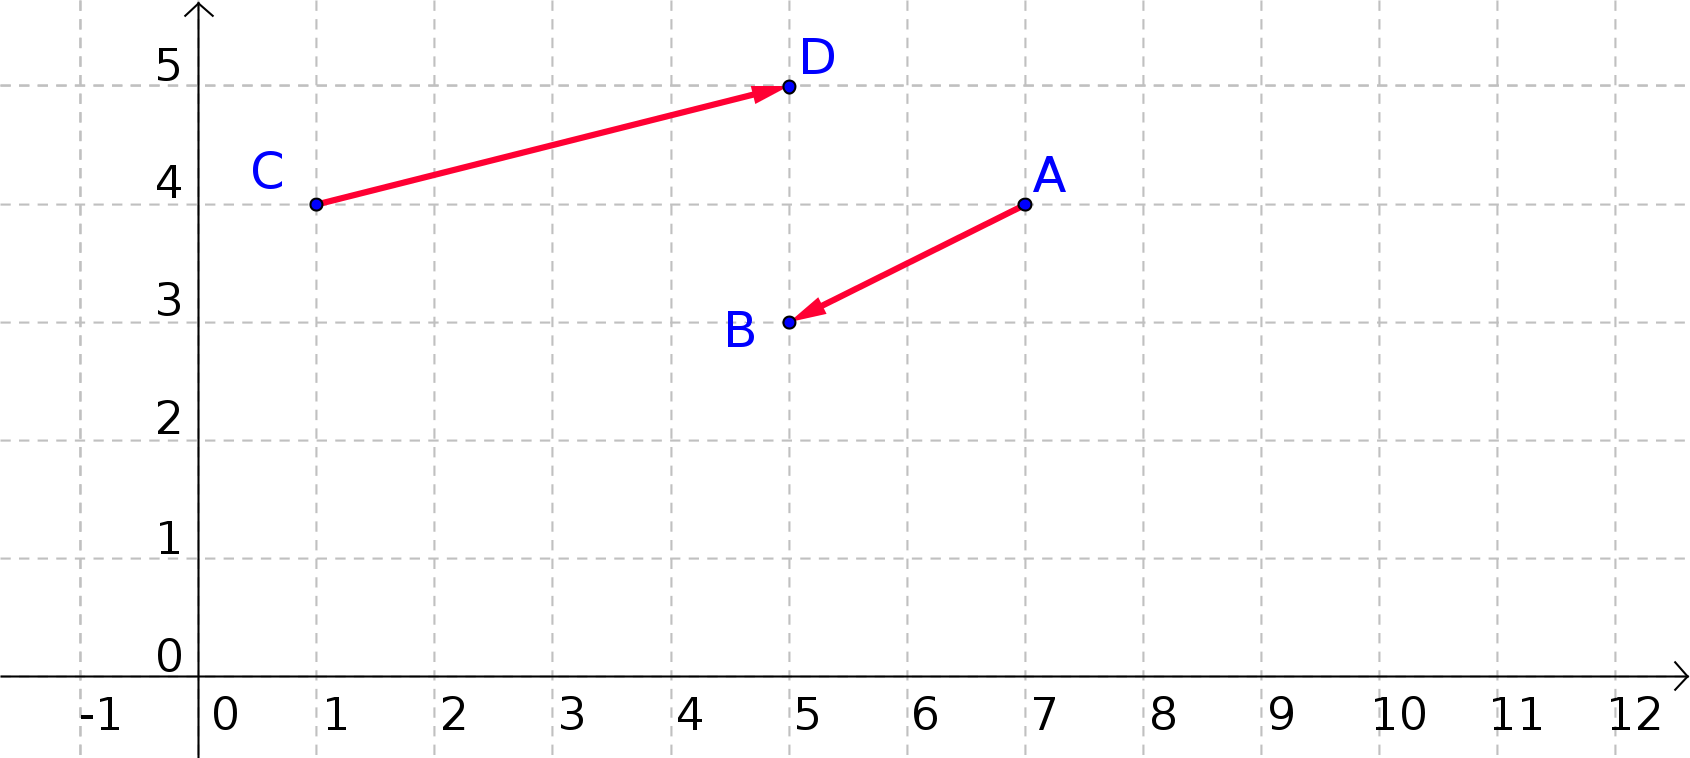
\includegraphics[width=0.5\textwidth]{Philippe/Figures_Philippe/vecteurs_4_5.png}
                \end{center}
            \end{question}
            \begin{reponses}
                \item[true] -9
                \item[false] -21
                \item[false] -55
                \item[false] -7 
            \end{reponses}
            %%%%%%%%%%%%%%%%%%%%%%%%%%%%%%%%%%%%%
            \begin{question}{1205}{Vecteurs}{2}{1220}
                Calculez le produit scalaire des vecteurs $\vec{A}=(4;2;1)$ et $\vec{B}=(1;0;6)$.
            \end{question}
            \begin{reponses}
                \item[true] 10
                \item[false] 11
                \item[false] 42
                \item[false] 14
            \end{reponses}
            %%%%%%%%%%%%%%%%%%%%%%%%%%%%%%%%%%%%%
            \begin{question}{1205}{Vecteurs}{2}{1217,31,1213}
                Que vaut le produit scalaire entre les deux vecteurs ci-dessous?
                \begin{figure}
                    \centering
                    \begin{tikzpicture}[scale=3, axis/.style={->,blue,thick}, vector/.style={-stealth,red,very thick}, vector guide/.style={dashed,red,thick}]
                        \coordinate[label=below  left:O] (O) at     (0cm,0cm);
                        \coordinate[label=below  left:] (x) at     (1cm,0cm);
                        \draw[axis] (0,0) -- (1,0) node[anchor=north         east]{$x$};
                        \draw[axis] (0,0) -- (0,1) node[anchor=north         west]{$y$};
                        \draw[-Stealth] (O) to [] ++ (480.0:2)         coordinate[label=above right:M] (M);
                        \draw[densely dotted] (O) to ["$x=-1$"] ++     (0:-1.0)     coordinate (Mx);
                        \draw[densely dotted] (Mx) to ["$y=\sqrt{3}$"]     ++     (90:1.73);
                        \pic["$\theta$", draw=red,->, angle radius =     12mm, angle eccentricity=1.3] {angle = x--O--M};
                    \end{tikzpicture} 
                    \begin{tikzpicture}[scale=3, axis/.style={->,blue,thick}, vector/.style={-stealth,red,very thick}, vector guide/.style={dashed,red,thick}]
                        \coordinate[label=below  left:O] (O) at     (0cm,0cm);
                        \coordinate[label=below  left:] (x) at     (1cm,0cm);
                        \draw[axis] (0,0) -- (1,0) node[anchor=north         east]{$x$};
                        \draw[axis] (0,0) -- (0,1) node[anchor=north         west]{$y$};
                        \draw[-Stealth] (O) to [] ++ (0:3)         coordinate[label=above right:M'] (M');
                        \draw[densely dotted] (O) to [] ++ (0:3.0)         coordinate (Mx);
                        \draw[densely dotted] (Mx) to [] ++ (90:0.0);
                        \draw (1,1) node[right]{$x'=3$, $y'=0$ };
                    \end{tikzpicture}
                \end{figure}
            \end{question}
            \begin{reponses}
                \item[true] \num{-3.0}
                \item[false] \num{-9.0}
                \item[false] \num{-10.92}
                \item[false] \num{-10.93}
            \end{reponses}
            \begin{question}{1205}{Vecteurs}{2}{1220}
                Le couplage d'un système ayant un moment magnétique $\vec{\mu}$ avec un champ magnétique $\vec{B}$ modifie l'énergie du système d'une quantité $\Delta E=-\vec{\mu}\cdot\vec{B}$. Que vaut cette quantité quand $\vec{\mu}=(2;-6;5)$ et $\vec{B}=(-3;1;-6)$?
            \end{question}
            \begin{reponses}
                \item[false] $E=7$
                \item[false] $E=-42$
                \item[false] $E=-7$
                \item[true] $E=42$
            \end{reponses}
            %%%%%%%%%%%%%%%%%%%%%%%%%%%%%%%%%%%%%
